\documentclass[12pt, a4paper, twoside, openright]{ppgccufsj}

\usepackage[english,portuguese]{babel} 
\usepackage[utf8]{inputenc}
%PACKAGE ADDED IN ORDER TO ENHANCE TYPOGRAPHY AT A VERY SMALL SCALE: 
%USING DIFFERENT TECHNIQUES, SUCH AS MARGIN KERNING (PROTRUSION), EXTRA KERNING, EXPANSION, TRACKING, AND SPACING
\usepackage[activate={true,nocompatibility},final,tracking=true,kerning=true,spacing=true,factor=1100,stretch=10,shrink=10]{microtype}
\usepackage[authoryear]{natbib}
\usepackage{lettrine}
\usepackage{lmodern}
\usepackage{times}
\usepackage{setspace}
\usepackage{xspace}
\usepackage{float}
\usepackage{color}
\usepackage{colortbl}
\usepackage{verbatim}
\usepackage{textfit}
\usepackage{latexsym}
\usepackage{multirow}
\usepackage{alltt}
\usepackage[T1]{fontenc}
\usepackage[verbose,left=25mm,right=25mm,top=30mm,bottom=30mm]{geometry}
\usepackage{ae}
\usepackage{fancyhdr}
\usepackage{fancybox}
\usepackage{multicol}
%\usepackage{listings}
\usepackage{subfig}
\usepackage{anysize}
\usepackage{setspace}
\usepackage{lastpage}
\usepackage{multirow}
\usepackage{longtable}
\usepackage{rotating}
\usepackage{caption}
\usepackage{placeins}
\usepackage{url}
\usepackage{xspace}
\usepackage{hyperref}  % GENERATES HYPERLINKS
\usepackage[chapter]{algorithm}
\usepackage{algpseudocode}

\hypersetup{colorlinks=true,debug=false,
  linkcolor=black,
  citecolor=black, 
  urlcolor=black,
  pdftitle={Thesis},
  pdfauthor={Vinicius Durelli},
  pdfsubject={thesis}}

\pdfcompresslevel=9

%%%%%%%%%%%%%%%%%%%%%%%%%%%%%%%%%%%%%%%%%%%%%%%%%%%%%%%%%%%%%%%%%%%%%%%%%%%%%%%%%%%%%%%%
\widowpenalty=10000
\clubpenalty=10000
\exhyphenpenalty=10000


%%%%%%%%%%%%%%%%%%%%%%%%%%---SPACING---%%%%%%%%%%%%%%%%%%%%%%%%%%%%%%%%%%%%%%%%%%%%%%%%%%
% spacing between words
\onehalfspacing
% spacing between figures, caption and text
\setlength{\abovecaptionskip}{0.223cm}
\setlength\textfloatsep{12pt}
\setlength\floatsep{12pt}  
% spacing between references
\setlength{\bibsep}{2.935pt}
%%%%%%%%%%%%%%%%%%%%%%%%%%%%%%%%%%%%%%%%%%%%%%%%%%%%%%%%%%%%%%%%%%%%%%%%%%%%%%%%%%%%%%%%

\headheight 17.1pt

\setcounter{secnumdepth} {3}
\setcounter{tocdepth} {3}
\definecolor{gray}{rgb}{0.7,0.7,0.7}


\begin{document}
%folder containing all images
\graphicspath{{imagens/}}	

\begingroup
\pagestyle{empty}
\thispagestyle{empty}

\ \vfill
\begin{center}
\begin{minipage}[c]{12cm}
\begin{center}
\hrulefill\\
%O TITULO DO TRABALHO DEVE SUBSTITUIR 'MODELO PARA DISSERTAÇÕES EM LATEX' 
\vspace{.5cm} {\Large\sf Modelo para Dissertações em \LaTeX}\\
\vspace{1.3cm}
%O NOME DO ALUNO DE MESTRADO DEVE SUBSTITUIR 'VINICIUS HUMBERTO SERAPILHA DURELLI'
\textbf{\large\textit{Vin\'icius Humberto Serapilha Durelli}}\\
\vspace{.5cm}
\hrulefill\\
\end{center}
\end{minipage}
\end{center}
\vfill

\cleardoublepage


%!TEX root = /Users/Viny/Desktop/Thesis/thesis_main.tex
\begin{flushright}
\begin{Sbox}
\begin{minipage}{8cm}
\footnotesize{
    SERVI\c{C}O DE P{\'O}S-GRADUA\c{C}{\~A}O DA UFSJ\\ \\
    Data de Dep{\'o}sito: \today \\ \\
    Assinatura:} \hrulefill
\end{minipage}
\end{Sbox}
\fbox{\TheSbox}
\end{flushright}

\vspace*{3cm}
\begin{center}
%O TITULO DO TRABALHO DEVE SUBSTITUIR 'MODELO PARA DISSERTAÇÕES EM LATEX'
{\Large\sf Modelo para Dissertações em \LaTeX}

%O NOME DO ALUNO DE MESTRADO DEVE SUBSTITUIR 'VINICIUS HUMBERTO SERAPILHA DURELLI'
\vspace*{2cm} \textbf{\textit{Vin\'icius Humberto Serapilha Durelli}}

\vspace*{2cm}
\textbf{Orientador:~\textit{Prof. Dr. John Winston Ono Lennon}}
\end{center}
\vspace*{3.5cm}
\begin{flushright}
\begin{minipage}{10cm}
	Monografia apresentada ao Departamento de Computação (DCOMP) da Universidade Federal de São João del Rei (UFSJ), 
	%para o Exame de Qualifica\c{c}{\~a}o, 
	como parte dos requisitos para obten\c{c}{\~a}o do t{\'\i}tulo de Mestre em Ci{\^e}ncia da Computa\c{c}{\~a}o.
\end{minipage}
\end{flushright}
\vspace*{2.5cm}
\begin{center}
\textbf{UFSJ - S{\~a}o João del Rei \\
        \ifcase\month\or
              Janeiro\or
              Fevereiro\or
              Mar\c{c}o\or
              Abril\or
              Maio\or
              Junho\or
              Julho\or
              Agosto\or
              Setembro\or
              Outubro\or
              Novembro\or
              Dezembro\fi/\the\year}
\end{center}
\cleardoublepage



%\newpage
%====THIS WHOLE BUNCH OF COMMANDS USED TO BE BEFORE THE ABSTRACT'S ENTRY====
\pagestyle{plain}
\thispagestyle{plain}
\renewcommand{\thepage}{\roman{page}}
\setcounter{page}{1}
%===========================================================================

\frontmatter
%\newpage
\begin{abstract}
  %!TEX root = /Users/Viny/Desktop/Thesis/thesis_main.tex

% CONTEXT/BACKGROUND: 
\lettrine{H}{igh-level} language virtual machines (HLL~VMs) have been playing a 
key role as a mechanism for implementing portable programming languages. 
Languages that run on these execution environments have many advantages over languages that are compiled to native code. 
These advantages have led HLL~VMs to gain broad acceptance in both academy and industry. 
% OBJECTIVE: 
However, 
much of the research in this area has been devoted to boosting the 
performance of these execution environments. 
Few efforts have attempted to introduce features that automate or 
facilitate some software engineering activities, 
including software testing. 
This research argues that 
HLL~VMs provide a reasonable basis for building an integrated software testing environment. 
% METHOD: 
To this end, 
two software testing features that build on the characteristics of  
a Java virtual machine (JVM) were devised. 
The purpose of the first feature is to automate weak mutation. 
Augmented with mutation support, 
the chosen JVM achieved speedups of as much as 89\% in comparison to a strong mutation tool. 
To support the testing of concurrent programs, 
the second feature is concerned with enabling the deterministic re-execution of Java programs and 
exploration of new scheduling sequences.
% RESULTS:  
% CONCLUSION:

\smallskip
\noindent \textbf{Keywords ---} software testing; mutation testing; weak mutation; record-and-playback mechanism; Maxine~VM; Java virtual machine.

% TO USE:
% The _recent_surge_in_ virtualization-related research has made its way not only into the security field but also into the malware scene, resulting in the creation of a new class of rootkits.

% EXAMPLE: "This dissertion investigates the possibility to improve the quality of text composi- tion. Two typographic extensions were examined: margin kerning and composing with font expansion."

\end{abstract}

\begin{resumo}
	%!TEX root = /Users/Viny/Desktop/Thesis/thesis_main.tex

\lettrine{M}{áquinas} virtuais de linguagens de programação têm desempenhado um papel importante como 
mecanismo para a implementação de linguagens de programação. 
Linguagens voltadas para esses ambientes de execução possuem  
várias vantagens em relação às linguagens compiladas. 
Essas vantagens fizeram com que tais ambientes de execução se tornassem amplamente utilizados pela 
indústria e academia. 
% Todavia, 
% a maioria dos 
% estudos nessa área têm sido dedicados a aprimorar o desempenho desses ambientes de execução. 
% Poucos esforços têm enfocado o desenvolvimento de funcionalidades 
% que automatizem ou facilitem a 
% condução de atividades de engenharia de software, 
% incluindo atividades de teste de software.
Entretanto, 
a maioria dos 
estudos nessa área têm se dedicado a aprimorar o desempenho desses ambientes de execução e poucos têm enfocado o desenvolvimento de funcionalidades 
que automatizem ou facilitem a 
condução de atividades de engenharia de software, 
incluindo atividades de teste de software. 
Este trabalho apresenta indícios de que   
máquinas virtuais de linguagens de programação podem apoiar a criação de ambientes de teste de software integrado. 
Para tal, 
duas funcionalidades que tiram proveito das características de uma máquina virtual Java 
foram desenvolvidas. 
O propósito da primeira funcionalidade é automatizar a condução de atividades de mutação fraca. 
Após a implementação de tal funcionalidade na máquina virtual Java selecionada, 
observou-se um desempenho até 89\% melhor em relação a uma ferramenta de mutação forte. 
% A fim de apoiar o teste de programas concorrentes, 
% a segunda funcionalidade possibilita que programas concorrentes sejam re-executados de forma determinística 
% e que novas sequências de escalonamento sejam automaticamente exploradas.  
A fim de apoiar o teste de programas concorrentes, 
a segunda funcionalidade permite reexecutá-los de forma determinística 
além de automatizar a exploração de que novas sequências de escalonamento.
 
\smallskip
\noindent \textbf{Palavras-chave ---} teste de software; teste de mutação; mutação fraca; mecanismo de record\--and\--playback; Maxine~VM; máquina virtual Java.

\end{resumo}

%**************************  INDEX ***********************************************
\microtypesetup{protrusion=false} % disables protrusion locally in the document
\newpage
\tableofcontents
\listoffigures
\listoftables
\microtypesetup{protrusion=true} % enables protrusion

% \newpage
\onehalfspace

\pagestyle{fancy}
\fancyfoot[C]{\thepage}
\fancyhead[R]{\leftmark}
\lhead{}            
\chead{}
\let\cite=\citep

%*******************************************************************************

\renewcommand{\thepage}{\arabic{page}}
\endgroup
\mainmatter
\setcounter{page}{1} 
\let\cite=\citep

%********************  INTRODUCAO   **************************************
% ----------------------------------------------------------
\chapter[Introdução]{Introdução}

Parte inicial do texto, que tem como objetivo elucidar os principais conceitos necessários para compreender os objetivos da pesquisa e outros elementos necessários para apresentar o tema do trabalho \citep{the_craft_of_research}. É importante que a introdução seja clara e convincente. 

A equipe de desenvolvimento e manutenção da classe PPGCCUFSJ e do modelo para teses e dissertações em \LaTeX\ utilizando a classe PPGCCUFSJ é integralmente composta pelas pessoas listadas abaixo. Atualmente, o propósito da equipe é garantir a sustentabilidade deste modelo, tendo autonomia para implementar novos recursos, efetuar compatibilizações necessárias em decorrência de alterações de normas da ABNT e/ou normas e padrões estabelecidos pela comissão de pós-graduação da UFSJ. 

\textbf{Programação}

\begin{itemize}
	\item Vinicius H. S. Durelli -- \url{durelli@ufsj.edu.br}
\end{itemize}

\textbf{Normalização e Padronização}

\begin{itemize}
	\item Vinicius H. S. Durelli -- \url{durelli@ufsj.edu.br}
\end{itemize}
	
O objetivo do presente trabalho é apresentar a classe PPGCCUFSJ e o modelo para teses e dissertações em \LaTeX\ utilizando a classe PPGCCUFSJ. 
A expectativa é que a classe PPGCCUFSJ e o modelo proposto auxiliem no aprimoramento da qualidade dos trabalhos acadêmicos produzidos pelos alunos de pós-graduação da UFSJ.
	


%********************  DESENVOLVIMENTO   *********************************
\chapter{Desenvolvimento}\label{cap_exemplos}

Este capítulo é parte principal da dissertação e deve conter a exposição ordenada e detalhada do assunto. 
Divide-se em seções e subseções, 
em conformidade com a abordagem do tema e do método, abrangendo: 
revisão bibliográfica, materiais e métodos, técnicas utilizadas, resultados obtidos e discussão.

O conteúdo deste documento visa apresentar um tutorial para utilização da classe PPGCCUFSJ, utilizando a estrutura de trabalhos acadêmicos, 
mas por questões didáticas adotou-se capítulo, seções e subseções diferentes das usualmente utilizadas.

\section{Classe PPGCCUFSJ e modelo de trabalho de acadêmico}

A classe PPGCCUFSJ é uma derivada de um antigo modelo utilizado no Instituto de Ciências Matemáticas e de Computação (ICMC) de São Carlos, Universidade de São Paulo (USP):

O objetivo do projeto é disponibilizar um modelo em \LaTeX\  para a elaboração de trabalhos acadêmicos (dissertação, trabalho de conclusão de curso (TCC), dentre outros) em conformidade com as normas do departamento de Ciência da Computação (DCOMP) da UFSJ. 

Este documento e seu código fonte são exemplos de uso da classe PPGCCUFSJ e do pacote \textsf{natbib}.

\section{Codificação dos arquivos: UTF8}

A codificação \texttt{UTF8} deve ser utilizada para todos os arquivos. 
Utilize a mesma codificação nos documentos que escrever, 
incluindo nos arquivos de base bibliográficas |.bib|. 
Para tanto, o arquivo \texttt{main.tex} deve conter o seguinte pacote:
\begin{verbatim}
\usepackage[utf8]{inputenc}	 
\end{verbatim}

\section{Tabelas}

As tabelas e os quadros apresentam os dados de modo resumido, 
oferecendo uma visão geral do conteúdo em questão, 
visando facilitar a compreensão do fenômeno em estudo. 
A diferença básica entre ambas está relacionada ao conteúdo e a formatação. 
Um exemplo de tabela é mostrado na página seguinte (Tabela~\ref{tab:descriptive_statistics_treatment}).\footnote{
A Tabela~\ref{tab:descriptive_statistics_treatment} foi extraída de \citet{please_please_me}.
}

\begin{table}[!htb]
	\caption{Sumário das características do grupo de tratamento~\citep{please_please_me}.\label{tab:descriptive_statistics_treatment}}
	\begin{center}
		\footnotesize
		\tabcolsep=0.11cm
		\begin{tabular}{ l | r | r | r | r |}
		 \cline{2-5}
		 &\multicolumn{4}{c|}{\textbf{Overview of the Treatment Group}} \\
		 \cline{2-5}
		 \multicolumn{1}{ l |}{\textbf{}} & \multicolumn{1}{c|}{\textbf{Google Play Reviews}} & \multicolumn{1}{c|}{\textbf{Rating}} & 
		 \multicolumn{1}{c|}{\textbf{Lifespan}} & \multicolumn{1}{c|}{\textbf{Commits}} \\
		\hline
		\multicolumn{1}{| r |}{\textbf{Max}} & 624,366 & 4.8 & 2,976 & 11,049 \\
		\hline
		\multicolumn{1}{| r |}{\textbf{Min}} & 91 & 3 & 759 & 31 \\
		\hline
		\multicolumn{1}{| r |}{\textbf{Mean}} & 31,658.4 & 4.27 & 1,873.80 & 2,704.53\\
		\hline
		\multicolumn{1}{| r |}{\textbf{Trimmed}} & 7,389.04 & 4.35 & 1,895.29 & 2,318.67 \\
		\hline
		\multicolumn{1}{| r |}{\textbf{Median}} & 3,523.0 & 4.4 & 2,113.5 & 1,682.5 \\
		\hline
		\multicolumn{1}{| r |}{\textbf{Std Dev}} & 113,831.38 & 0.42 & 641.29 & 2,748.98 \\
		\hline
		\multicolumn{1}{| r |}{\textbf{MAD$^\ddag$}} & 4,918.53 & 0.22 & 491.48 & 2,029.68 \\
		\hline
		\multicolumn{5}{| l |}{$^\ddag$MAD stands for median absolute deviation.} \\
		\hline
		\end{tabular}
	\end{center}
\end{table}

\section{Figuras} 

Figuras podem ser criadas diretamente em \LaTeX ou podem ser 
incorporadas por meio de um arquivo externo, 
como é o caso da Figura~\ref{fig:execution_flow}.\footnote{A Figura~\ref{fig:execution_flow} foi extraída de \citet{speeding_up_mutation_testing}.} 
É importante que sejam utilizadas imagens vetoriais no formato PDF. 
Com isso, o tamanho do arquivo final do trabalho será menor e as imagens terão uma apresentação melhor, 
principalmente quando impressas, uma vez que imagens vetoriais são perfeitamente escaláveis para qualquer dimensão. 

\begin{figure}[H]
 \center
 \scalebox{0.6}{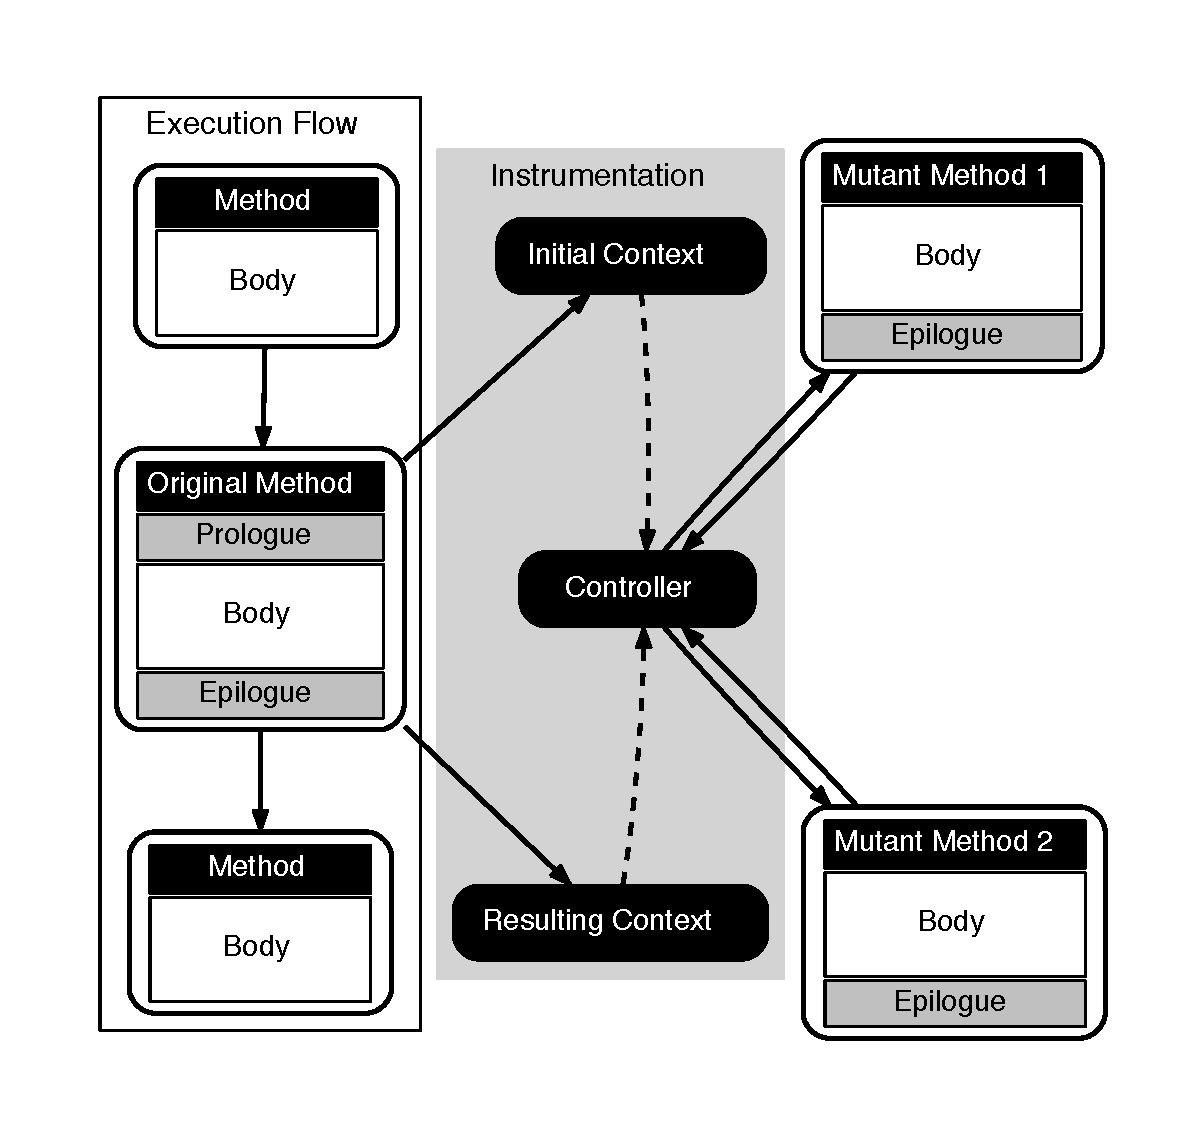
\includegraphics{execution_flow_overview}}
 \caption{Visão geral do pré-processamento de métodos originais antes de serem compilados pela máquina virtual Java.}
 \label{fig:execution_flow}
\end{figure}

\section{Diferentes idiomas e hifenizações}
\label{sec-hifenizacao}

Para usar hifenizações de diferentes idiomas, inclua nas opções do documento o
nome dos idiomas que o seu texto contém. Os usuários da classe PPGCCUFSJ devem utilizar:

\begin{verbatim}
\usepackage[english, %idioma adicional
portuguese]{babel} 
\end{verbatim}

Desta forma o texto deverá ser escrito idioma português-brasileiro (\texttt{brazil}), podendo ter citações em inglês.
Os idiomas português-brasileiro (\texttt{brazil}) e inglês são incluídos automaticamente pela classe.



%******************  REFERENCIAS  *****************************************
\microtypesetup{protrusion=false,tracking=false,kerning=false,spacing=false}
\bibliographystyle{ppgccufsj}
\bibliography{referencias}
\microtypesetup{protrusion=true,tracking=true,kerning=true,spacing=true}
%***************************************************************************
\end{document}

